\documentclass[UTF8,zihao=-4]{ctexart}
\usepackage[a4paper,margin=2.5cm]{geometry}
\usepackage{amsmath, amssymb, amsthm}
\usepackage{bm}
\usepackage{hyperref}
\usepackage{graphicx}
\usepackage{caption}
\usepackage{listings}
\usepackage{xcolor}
\usepackage{float}
\usepackage{booktabs}
\usepackage{longtable}
\usepackage{multirow}
\usepackage{placeins}
\graphicspath{{figures/}}

% 代码样式
\lstdefinestyle{code}{
  basicstyle=\ttfamily\small,
  numbers=left,
  numberstyle=\tiny,
  numbersep=8pt,
  keywordstyle=\color{blue},
  commentstyle=\color{teal!70!black},
  stringstyle=\color{orange!70!black},
  showstringspaces=false,
  breaklines=true,
  frame=single,
  framerule=0.3pt,
  rulecolor=\color{black!15}
}
\lstset{style=code}

\title{检索增强生成(RAG)体系:信息注入、向量管线与微调融合}
\author{}
\date{\today}

\begin{document}
\maketitle

\section{检索增强原理与信息注入机制}
\subsection{核心理念}
检索增强生成(Retrieval-Augmented Generation, RAG)通过外部知识库弥补大模型的知识盲点和时效性问题。其基本流程如图\ref{fig:rag_pipeline_cn} 所示:用户查询首先编码为向量,经过向量搜索检索相关文档,再将检索到的证据与原始查询拼接或重写,最后输入到 LLM 生成带来源的回答。
\begin{figure}[H]
  \centering
  
\includegraphics[width=0.9\textwidth]{rag_pipeline.png}
  \caption{RAG 推理流水线:查询嵌入、向量检索、上下文融合、LLM 带引用回答。}
  \label{fig:rag_pipeline_cn}
\end{figure}

\subsection{检索与生成的闭环}
\begin{itemize}
  \item \textbf{双向依赖:} 检索结果的质量直接决定生成上限,而生成阶段的指令(如引用要求、回答结构)反过来影响对证据的需求。
  \item \textbf{信息注入策略:} 常见方法包括直接拼接(concatenation)、模板化摘要(structured prompt)、与查询融合(query rewriting)以及面向段落的排序权重(re-ranking)。
  \item \textbf{反馈机制:} 通过生成结果对检索阶段提供反馈(如未找到答案时触发“虚无检索”或改写查询),形成自适应回路。
\end{itemize}

\subsection{典型架构拓扑}
\begin{longtable}{p{3cm}p{5cm}p{6cm}}
\toprule
类型 & 描述 & 应用场景 \\
\midrule
经典 RAG & 查询 $\rightarrow$ 检索 $\rightarrow$ 拼接 $\rightarrow$ 生成 & FAQ、知识库问答、客服机器人 \\
双塔 + 重排 & 首先使用轻量向量检索,然后使用交叉编码器重排 & 法律、医疗等需要高精度匹配的场景 \\
自适应检索 & LLM 根据需要决定检索次数和查询改写 & 工具增强型 Agent、实时信息查询 \\
文档先摘要 & 对大文档预生成摘要或结构化节点,查询时检索摘要再回溯全文 & 长文档阅读、报告生成 \\
\bottomrule
\end{longtable}

\section{文档分块与向量嵌入(Embeddings)}
\subsection{分块策略}
在向量化之前需要将文档切分为语义单元,图\ref{fig:chunk_flow_cn} 展示了从原始文档到向量库的步骤。
\begin{figure}[H]
  \centering
  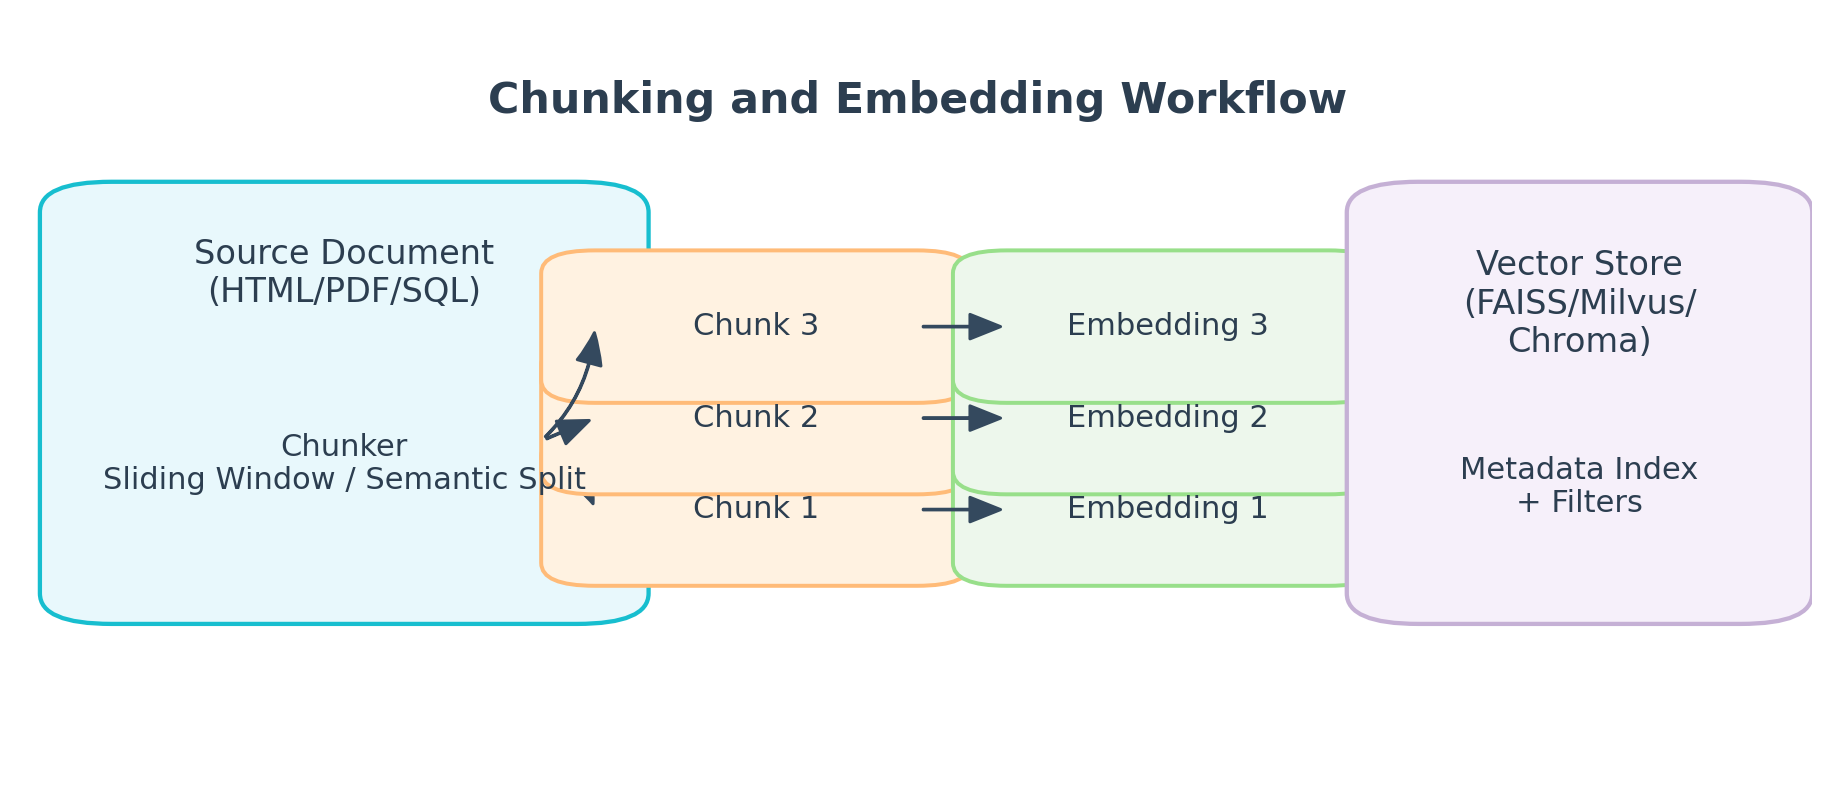
\includegraphics[width=0.9\textwidth]{chunk_embedding.png}
  \caption{分块与嵌入工作流:原始文档经滑动窗口/语义分段生成 Chunk,再编码为向量并存入向量库。}
  \label{fig:chunk_flow_cn}
\end{figure}
常用分块策略:
\begin{itemize}
  \item \textbf{固定窗口 + 重叠:} 适合结构化程度较低的文本,一般设置 200--512 token 的窗口,重叠 10--20\% 防止断句。
  \item \textbf{语义分段:} 基于句子、段落或语义相似度分段,采用 TextTiling、语义聚类、标题检测等算法。
  \item \textbf{结构化切分:} 对表格、代码、知识图谱等,按字段或节点组织,保留元信息。
\end{itemize}

\subsection{嵌入模型选择}
\begin{itemize}
  \item \textbf{通用模型:} 如 OpenAI \texttt{text-embedding-3-large}、bge-large、m3e 等,在多语言场景表现稳定。
  \item \textbf{领域模型:} 针对法律、医疗、金融的专用模型,通常由开源模型 LoRA 微调(如 BAAI/bge-law)。
  \item \textbf{稀疏表示:} 结合 BM25、ColBERT 等稀疏/混合检索方式,补充关键词匹配能力。
\end{itemize}

\subsection{嵌入与元数据}
每个 chunk 向量通常关联以下元数据:
\begin{itemize}
  \item 文档 ID、段落编号、标题、创建时间、权重、标签;
  \item 结构化字段(如产品类别、地理位置)用于过滤;
  \item 原始文本以及压缩摘要,用于模型阅读或展示。
\end{itemize}
合理设计元数据可以在检索阶段进行布尔过滤、时间筛选、权重排序,提高结果相关性。

\subsection{批量编码示例}
\begin{lstlisting}[language=Python,caption={使用 SentenceTransformers 批量编码文档 chunk}]
from sentence_transformers import SentenceTransformer
from datasets import load_dataset

model = SentenceTransformer("BAAI/bge-large-zh-v1.5")
dataset = load_dataset("json", data_files="chunks.jsonl")["train"]

def encode_batch(batch):
    embeddings = model.encode(batch["text"], batch_size=64, show_progress_bar=False, normalize_embeddings=True)
    batch["embedding"] = [emb.tolist() for emb in embeddings]
    return batch

encoded = dataset.map(encode_batch, batched=True, batch_size=512)
encoded.to_parquet("chunks_with_embeddings.parquet")
\end{lstlisting}

\section{向量数据库(FAISS, Milvus, Chroma)}
\subsection{核心功能对比}
\begin{longtable}{p{3cm}p{4cm}p{6cm}}
\toprule
引擎 & 特点 & 适用场景 \\
\midrule
FAISS & Facebook AI 研发,支持 IVF、HNSW、PQ 等索引;内存型高性能 & 单机/内存充足,需自定义部署与调优的工程团队 \\
Milvus & 云原生架构,支持分布式存储、向量+标量过滤、CDC;提供 Milvus Lite & 企业级多副本、高可用、与对象存储集成 \\
Chroma & 轻量级、嵌入式,支持 SQL API、持久化到 SQLite/Postgres & 快速原型、桌面应用、少量数据场景 \\
\bottomrule
\end{longtable}

\subsection{索引策略}
\begin{itemize}
  \item \textbf{暴力检索(Flat):} 精确但耗时,适合小规模或精确召回阶段(如重排前筛选)。
  \item \textbf{近似最近邻(ANN):} IVF、HNSW、ScaNN 等方法,通过分桶或图结构实现 $O(\log n)$ 检索。
  \item \textbf{量化压缩:} 产品量化(PQ)、OPQ、LSQ 等降低内存占用,适合海量向量。
\end{itemize}
在工程实践中常采用“双阶段”策略:先用 ANN 快速召回,再使用精确距离或交叉编码器重排。

\subsection{Milvus 查询示例}
\begin{lstlisting}[language=Python,caption={在 Milvus 中执行向量检索}]
from pymilvus import connections, Collection, utility
import numpy as np

connections.connect("default", uri="http://localhost:19530")

if not utility.has_collection("rag_chunks"):
    raise RuntimeError("Collection rag_chunks does not exist")

collection = Collection("rag_chunks")
collection.load()

query_vector = np.load("query_embedding.npy")
search_params = {"metric_type": "IP", "params": {"nprobe": 32}}

results = collection.search(
    data=[query_vector.tolist()],
    anns_field="embedding",
    param=search_params,
    limit=5,
    output_fields=["doc_id", "text", "score", "tags"]
)

for hit in results[0]:
    print(hit.id, hit.distance, hit.entity.get("doc_id"), hit.entity.get("tags"))
\end{lstlisting}

\section{RAG 与 Fine-tuning 的结合方式}
\subsection{互补关系}
\begin{itemize}
  \item \textbf{RAG 解决知识更新:} 通过检索引入最新数据,降低微调频率与推理成本。
  \item \textbf{微调提升生成风格:} 对 RAG 输出的格式、语气、推理深度进行定制化;
  \item \textbf{联合优化:} 通过微调模型使其更善于阅读检索上下文、引用来源并区分多段证据。
\end{itemize}

\subsection{常见组合方案}
\begin{itemize}
  \item \textbf{Instruction Tuning + RAG:} 先对模型进行指令微调,使其遵守回答模板,再用 RAG 注入实时知识。
  \item \textbf{Retriever Fine-tuning:} 使用对比学习(如 Contriever、ColBERT)对嵌入模型微调,提高召回质量。
  \item \textbf{Generator Fine-tuning:} 采用 RAG 样本(问题、证据、答案)对 LLM 做监督微调或 DPO,提升引用准确性。
  \item \textbf{End-to-End RAG Fine-tuning:} 在检索和生成之间引入可微分模块(如 RETRO、Atlas)实现联合训练。
\end{itemize}

\subsection{训练数据构建}
\begin{itemize}
  \item \textbf{构造三元组:} $(q, d^+, d^-)$ 对,用于训练嵌入模型;$d^-$ 可来自随机抽样或难负样本挖掘。
  \item \textbf{证据标注:} 对生成答案标记引用的文档和段落,为监督微调提供对齐信号。
  \item \textbf{自监督数据:} 通过让模型对检索内容回答问题,再将模型自评得分用于强化学习或过滤低质量样本。
\end{itemize}

\subsection{组合评估策略}
\begin{longtable}{p{3cm}p{3cm}p{4cm}p{4cm}}
\toprule
指标类别 & 指标 & 关注点 & 工具 \\
\midrule
检索指标 & Recall@k、MRR、nDCG & 覆盖率与排序质量 & BEIR、LlamaIndex Eval \\
生成指标 & BLEU、ROUGE、Factuality & 表达质量与真实性 & GPT-judge、FactScore \\
引用指标 & Precision@k(引用)、覆盖度 & 引用准确性、幻觉率 & 自定义正则表达式、Heuristic \\
端到端 & 用户反馈、工单转化率 & 业务 KPI & A/B Testing、在线实验 \\
\bottomrule
\end{longtable}

\section*{实践建议}
\begin{itemize}
  \item 设计结构化 Prompt,将检索到的证据标号呈现,指导模型引用具体段落。
  \item 定期刷新向量库与嵌入模型,针对新增数据执行增量索引与热度调节。
  \item 使用离线与在线评测联动,确保检索与生成的优化同步推进。
  \item 为 RAG + 微调流程配置监控,跟踪检索命中率、回答准确率与安全误报。
\end{itemize}

\section*{参考文献}
\begin{itemize}
  \item Lewis et al. ``Retrieval-Augmented Generation for Knowledge-Intensive NLP Tasks.'' NeurIPS, 2020.
  \item Izacard et al. ``Few-shot Learning with RETRO.'' arXiv, 2022.
  \item Humeau et al. ``Poly-encoders: Architectures and Pre-training Strategies for Fast and Accurate Multi-sentence Scoring.'' ICLR, 2020.
  \item Xu et al. ``BGE: BE Better in Embedding.'' arXiv, 2023.
  \item Chen et al. ``Atlas: Few-shot Learning with Retrieval Augmented Language Models.'' ICML, 2022.
\end{itemize}

\end{document}

